\section{Divisori di frequenza}
\subsection{Montaggio e verifica}
Si è innanzitutto realizzato il circuito in \fig{div} utilizzando l'integrato SN74LS93 (un ripple counter costituito da quattro JK flip-flop), mettendo uno degli ingressi di reset ($R_{0,1}$) a terra, per poi verificarne visivamente il corretto funzionamento inviando un clock lento ($\sim \SI{1}{\Hz}$) ed osservando i LED (e dunque gli output dei flip-flop) "contare" ciclicamente da 0 a 15.

\begin{figure}[h]
	\centering
	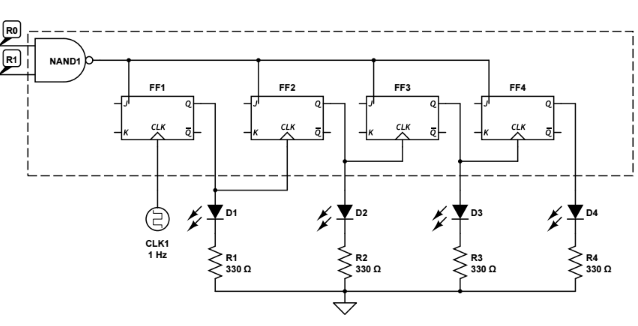
\includegraphics[scale=0.8]{divisori.png}
	\caption{Circuito divisore}
	\label{fig:div}
\end{figure}

\begin{figure}[h]
	\centering
	\begin{minipage}{0.47\textwidth}
		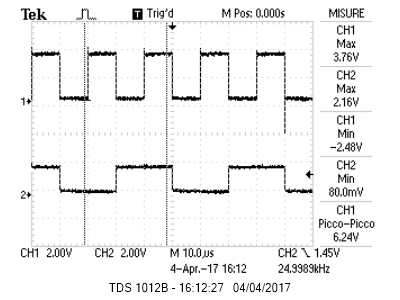
\includegraphics[scale=0.8]{divisore_2x.png}
		\\
		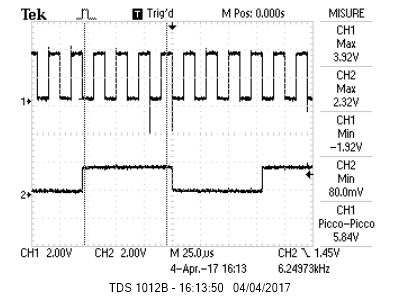
\includegraphics[scale=0.8]{divisore_8x.png}
	\end{minipage}
	\begin{minipage}{0.47\textwidth}
		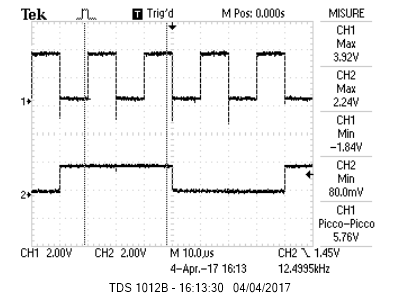
\includegraphics[scale=0.8]{divisore_4x.png}
		\\
		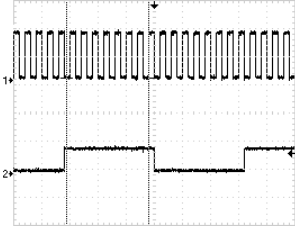
\includegraphics[scale=0.8]{divisore_16x.png}
	\end{minipage}
	\caption{Output dei quattro flip-flop del divisore (CH2) e segnale di clock (CH1).}
	\label{fig:divout}
\end{figure}
